\documentclass[11pt,a4paper]{article}

\usepackage[T1]{fontenc}
\usepackage{lmodern}
\usepackage[margin=2.5cm]{geometry}
\usepackage{microtype}
\usepackage{amsmath,amssymb}
\usepackage{booktabs}
\usepackage{graphicx}
\usepackage{adjustbox}
\usepackage{float}
\usepackage[labelfont=bf,font=small]{caption}
\usepackage{subcaption}
\usepackage{enumitem}
\usepackage{xcolor}
\usepackage{listings}
\usepackage[round,authoryear]{natbib}
\usepackage[colorlinks=true,linkcolor=blue!50!black,citecolor=blue!50!black,urlcolor=blue!50!black]{hyperref}

\definecolor{codebg}{RGB}{247,247,247}
\lstset{
  language=Python, basicstyle=\ttfamily\footnotesize, backgroundcolor=\color{codebg},
  keywordstyle=\color{blue!60!black}\bfseries, commentstyle=\color{green!40!black}\itshape,
  stringstyle=\color{red!50!black}, frame=single, rulecolor=\color{black!15},
  breaklines=true, columns=fullflexible, showstringspaces=false, aboveskip=6pt, belowskip=6pt
}

\newcommand{\Q}[1]{\textsc{[Q#1]}}
\newcommand{\code}[1]{\texttt{#1}}
\setlength{\parskip}{0.35em}
\setlength{\emergencystretch}{2em}

\title{\textbf{Spreads, Liquidity Timing and Order-Book Gaps:\\
An Empirical Study of Level-2 Snapshots for Five Chinese A-Shares}\\[0.6em]
\large Data Team --- Written Test B}
\author{Tianzuo Hu\\[0.2em]\normalsize Cornell University}
\date{November 2026}

\begin{document}
\maketitle

\begin{abstract}
\noindent
We assemble three days (4--6 January 2021) of 3-second limit-order-book snapshots and 15-second
trade records for five anonymised Chinese A-shares into a single, validated panel of 71{,}085
observations, derive snapshot-level and one-minute features, and use them to study three
aspects of market microstructure. First, the quoted spread is governed by the \emph{relative} tick
size: low-priced stocks sit at the one-tick floor more than 80\% of the time, whereas the two
high-priced stocks have median spreads of 2 and 4 ticks. When the spread widens, more than 91\%
of episodes are \emph{one-sided} (only one best quote moves outward), consistent with the
depletion of a single best queue rather than a symmetric withdrawal of liquidity. Second,
trading activity follows the familiar intraday pattern: the first 30 minutes account for 26--29\%
of daily turnover (against 12.7\% under a uniform profile), and the absolute one-minute return is
positively related to one-minute turnover (correlation 0.34--0.37). Third, the most recent trade
price sits at the best bid or best ask in 80--99\% of fresh prints; when the price is forward-filled
between prints, its position relative to the book spreads out, and it does so most for the
small-tick stocks. Finally, we detect 17{,}925 \emph{free-hole additions} (new orders posted at
previously empty interior price levels). Almost all of them (95\%) occur in the two stocks whose
displayed books contain gaps. They are most common at level 2, and half of them have no more
than 2{,}100 shares queued ahead.
\end{abstract}

\tableofcontents
\vspace{0.5em}
\noindent\textit{Navigation.} Every answer is tagged with the question it addresses, e.g.\ \Q{3b}.
All numbers are produced by the accompanying script \code{analysis.py}, which also writes the
tables included below; nothing was transcribed by hand.

%==========================================================================================
\section{Data and validation}\label{sec:data}

\paragraph{Sources.} For each stock ($i=1,\dots,5$) and day ($d\in\{20210104,20210105,20210106\}$) we
have a \emph{snapshot} file (best five bid/ask prices and quantities, every 3\,s, 4{,}739 rows per
stock-day) and a \emph{trade} file (volume, turnover and last traded price aggregated over 15\,s,
947 rows per stock-day). The files are stored as \code{data/\{snapshot,trade\}/\{date\}/\{id\}.csv}
(this differs slightly from the naming pattern given in the task description). Sessions run from
09:30 to 11:30 and from 13:00 to 14:57. The closing call auction (14:57--15:00) is not part of the
sample.

\paragraph{Integrity checks.} Before any analysis the script asserts that (i)~every stock-day has
exactly 4{,}739 snapshots and 947 trade records; (ii)~$\text{bid1p}<\text{ask1p}$ in every snapshot
(no locked or crossed books); (iii)~the bid ladder is strictly decreasing and the ask ladder strictly
increasing; (iv)~all prices lie on the CNY~0.01 tick grid; (v)~all displayed quantities are strictly
positive and nothing is missing; and (vi)~every trade timestamp also occurs in the snapshot
file. All checks pass. Price comparisons later in the analysis (spread changes, last-price
categories and free holes) are done on integer tick counts ($\text{price}/0.01$) so that
floating-point error cannot affect them.

\begin{table}[H]
\centering\small
\caption{Price level of the five stocks (mid-quote, CNY, all three days).}
\label{tab:desc}
\begin{tabular}{lrrr}
\toprule
Stock & Mean mid-price & Min & Max \\
\midrule
Stock 1 & 5.23 & 5.17 & 5.33 \\
Stock 2 & 100.28 & 97.04 & 104.74 \\
Stock 3 & 21.33 & 20.61 & 22.30 \\
Stock 4 & 11.65 & 11.20 & 12.09 \\
Stock 5 & 210.94 & 187.12 & 222.05 \\
\bottomrule
\end{tabular}

\end{table}

The stocks cover a wide price range (Table~\ref{tab:desc}), from about CNY~5 to CNY~211. Because
the tick is CNY~0.01 for all of them, one tick is worth about 19 basis points for stock~1 and less
than half a basis point for stock~5. This difference in \emph{relative tick size}
\citep{harris1994,dayri2015} explains most of the cross-sectional differences reported below.

%==========================================================================================
\section{Data assembly (Questions 1, 2 and 4)}\label{sec:assembly}

\paragraph{\Q{1} Combined snapshot panel.} The 15 snapshot files are read in a loop, concatenated
and sorted by \code{[id, date, time]}. Times are zero-padded strings (\code{"09:30:03"}), so
lexicographic order coincides with chronological order. The result, \code{df\_snapshot}, has
71{,}085 rows ($5\times3\times4{,}739$) and 23 columns.

\paragraph{\Q{2} Wide table of ask1p.} Setting the index to \code{(date, time, id)} and calling
\code{unstack("id")} gives one row per unique (date, time) and one column per stock. The table
has $3\times4{,}739 = 14{,}217$ rows and no missing cells, which confirms that the five stocks share
the same snapshot clock. Table~\ref{tab:q2} shows the first rows.

\begin{lstlisting}
ask_wide = df_snapshot.set_index(["date", "time", "id"])["ask1p"].unstack("id")
\end{lstlisting}

\begin{table}[H]
\centering\small
\caption{\Q{2} First rows of the (date, time) $\times$ stock table of best ask prices.}
\label{tab:q2}
\begin{tabular}{llrrrrr}
\toprule
date & time & stock 1 & stock 2 & stock 3 & stock 4 & stock 5 \\
\midrule
20210104 & 09:30:03 & 5.33 & 99.20 & 21.22 & 11.25 & 188.17 \\
20210104 & 09:30:06 & 5.33 & 99.47 & 21.22 & 11.24 & 188.80 \\
20210104 & 09:30:09 & 5.33 & 99.58 & 21.24 & 11.24 & 188.08 \\
20210104 & 09:30:12 & 5.32 & 99.74 & 21.24 & 11.23 & 188.51 \\
20210104 & 09:30:15 & 5.32 & 99.80 & 21.19 & 11.23 & 188.45 \\
20210104 & 09:30:18 & 5.31 & 99.90 & 21.26 & 11.23 & 188.08 \\
\bottomrule
\end{tabular}

\end{table}

\paragraph{\Q{4a} Merge.} The 15 trade files are combined in the same way into \code{df\_trade}
(14{,}205 rows). We left-join them onto \code{df\_snapshot} on \code{[id, date, time]} with
\code{validate="one\_to\_one"}. The merged frame \code{df} has 71{,}085 rows, exactly as many as
\code{df\_snapshot}. A separate inner join confirms that all 14{,}205 trade timestamps find a
matching snapshot.

\paragraph{\Q{4b} Forward fill.} \code{last} is forward-filled within each stock-day, so that
no price is carried from one stock to another or from one day to the next:
\begin{lstlisting}
df["last"] = df.groupby(["id", "date"])["last"].ffill()
\end{lstlisting} Before filling, 56{,}880 values are missing (the snapshots that
have no trade record). After filling, 60 remain: the first four snapshots of each stock-day
(09:30:03--09:30:12), which precede the first trade record at 09:30:15. We deliberately leave them
as \code{NaN}. Filling them backwards would use information from the future.

\paragraph{\Q{4c} Volume and amount.} The missing \code{volume} and \code{amount} values are set
to zero, because no trade record means no trading in the interval, and the columns are cast to
\code{int64}. All source values are already whole numbers (0 fractional entries), so the cast loses
nothing. Note that the first record of each day (09:30:15) is unusually large. It holds on
average 2.3\% (at most 3.9\%) of daily volume, which suggests that it also contains the
opening-auction match.

%==========================================================================================
\section{The bid--ask spread (Question 3)}\label{sec:spread}

\subsection*{\Q{3a} Distribution}

Table~\ref{tab:spreadcny} reports the requested percentiles of
$\text{bid\_ask\_sprd} = \text{ask1p}-\text{bid1p}$, both for the pooled sample and for each stock.
For the pooled sample, the spread equals the one-tick floor (CNY~0.01) from the 1st percentile up
to the median. It is 0.02 at the 75th percentile, 0.06 at the 90th, 0.10 at the 95th and 0.25 at the
99th; the mean is 0.028.

\begin{table}[H]
\centering\small
\caption{\Q{3a} Percentiles of the bid--ask spread (CNY).}
\label{tab:spreadcny}
\begin{adjustbox}{max width=\textwidth}
\begin{tabular}{lrrrrrrrrrr}
\toprule
Sample & 1\% & 5\% & 10\% & 25\% & 50\% & 75\% & 90\% & 95\% & 99\% & Mean \\
\midrule
All & 0.010 & 0.010 & 0.010 & 0.010 & 0.010 & 0.020 & 0.060 & 0.100 & 0.250 & 0.028 \\
Stock 1 & 0.010 & 0.010 & 0.010 & 0.010 & 0.010 & 0.010 & 0.010 & 0.010 & 0.020 & 0.010 \\
Stock 2 & 0.010 & 0.010 & 0.010 & 0.010 & 0.020 & 0.040 & 0.080 & 0.110 & 0.190 & 0.035 \\
Stock 3 & 0.010 & 0.010 & 0.010 & 0.010 & 0.010 & 0.010 & 0.010 & 0.020 & 0.030 & 0.011 \\
Stock 4 & 0.010 & 0.010 & 0.010 & 0.010 & 0.010 & 0.010 & 0.020 & 0.020 & 0.030 & 0.012 \\
Stock 5 & 0.010 & 0.010 & 0.010 & 0.020 & 0.040 & 0.090 & 0.170 & 0.240 & 0.470 & 0.070 \\
\bottomrule
\end{tabular}

\end{adjustbox}
\end{table}

The pooled distribution mixes stocks whose tick is economically very different, so we also
express the spread in ticks and in basis points of the mid-quote (Table~\ref{tab:spreadrel}). Following the usual definition \citep{eisler2012,dayri2015}, the
three low-priced stocks are \emph{large-tick} assets: their spread is pinned at one tick 83--98\% of
the time, and the relative spread (4.7--19.2\,bp at the median) is set by the tick itself rather than
by competition between liquidity providers. Stocks~2 and~5 are \emph{small-tick} assets: the spread
is one tick only 40\% and 23\% of the time, averages 3.5 and 7.0 ticks, and has a long right tail,
even though it is only about 2\,bp at the median. These two stocks account for most of the pooled
upper percentiles.

\begin{table}[H]
\centering\small
\caption{\Q{3a} Spread in ticks and in basis points of the mid-quote.}
\label{tab:spreadrel}
\begin{adjustbox}{max width=\textwidth}
\begin{tabular}{lrrrrrr}
\toprule
Stock & Mean price & Mean spread (ticks) & Share at 1 tick (\%) & 5\% (bp) & Median (bp) & 95\% (bp) \\
\midrule
Stock 1 & 5.23 & 1.02 & 97.70 & 18.92 & 19.18 & 19.29 \\
Stock 2 & 100.28 & 3.45 & 39.99 & 0.99 & 2.00 & 10.90 \\
Stock 3 & 21.33 & 1.13 & 90.31 & 4.56 & 4.72 & 9.39 \\
Stock 4 & 11.65 & 1.21 & 82.86 & 8.41 & 8.62 & 17.35 \\
Stock 5 & 210.94 & 7.04 & 22.85 & 0.46 & 1.88 & 11.21 \\
\bottomrule
\end{tabular}

\end{adjustbox}
\end{table}

\subsection*{\Q{3b} Spread widening}

Within each stock-day we compare every snapshot with the previous one. The first snapshot of a day
is never compared with the previous day. The transition 11:30:00\,$\to$\,13:00:03 is kept, because
these are consecutive snapshots in the data. A \emph{widening} is $\Delta\text{sprd}>0$. For each
widening we record whether bid1p fell \emph{and} ask1p rose (``Both''), or exactly one of the two
happened (``XOR''). Since a widening requires $\Delta\text{ask1p} > \Delta\text{bid1p}$, at least
one of the two events must occur, so Both $+$ XOR $=100\%$ (the script asserts this identity).

\begin{table}[H]
\centering\small
\caption{\Q{3b} Spread-widening events and how the two best quotes moved.}
\label{tab:widen}
\begin{tabular}{lrrrrr}
\toprule
Stock & Comparisons & Times widened & Widen rate (\%) & Both (\%) & XOR (\%) \\
\midrule
Stock 1 & 14{,}214 & 209 & 1.47 & 0.00 & 100.00 \\
Stock 2 & 14{,}214 & 4{,}394 & 30.91 & 8.01 & 91.99 \\
Stock 3 & 14{,}214 & 975 & 6.86 & 2.46 & 97.54 \\
Stock 4 & 14{,}214 & 1{,}261 & 8.87 & 1.98 & 98.02 \\
Stock 5 & 14{,}214 & 5{,}668 & 39.88 & 8.91 & 91.09 \\
All & 71{,}070 & 12{,}507 & 17.60 & 7.24 & 92.76 \\
\bottomrule
\end{tabular}

\end{table}

Table~\ref{tab:widen} shows the results. The spread widens in only 1.5\% of snapshot transitions for
stock~1 (209 times), but in 31\% and 40\% for stocks~2 and~5 (4{,}394 and 5{,}668 times). In every
stock the large majority of widenings, between 91\% and 100\%, are one-sided. Simultaneous
withdrawal on both sides accounts for at most 9\%, and never occurs for stock~1.

Table~\ref{tab:xor} splits the one-sided events further. For the large-tick stocks, most widenings
are a ``pure'' depletion: one best level disappears (it is consumed by a marketable order or
cancelled) while the opposite quote stays put. This covers 99\% of cases for stock~1 (split roughly
evenly between bid and ask), and 63\% and 76\% for stocks~3 and~4. For the small-tick stocks, 54--61\% of widenings are instead
\emph{shifts}: both quotes move in the same direction, but the leading side moves further. This is
what happens when the price drifts and liquidity on the trailing side is slow to follow. These
patterns are consistent with the view that spread dynamics are driven mainly by individual order
book events that hit one side of the book \citep{eisler2012}, and with the finding of
\citet{biais1995} that both quotes shift down (up) after large sales (purchases).

\begin{table}[H]
\centering\small
\caption{\Q{3b} Decomposition of one-sided widenings (\% of all widenings of the stock).}
\label{tab:xor}
\begin{tabular}{lrrrr}
\toprule
Stock & Bid down, ask flat & Ask up, bid flat & Both down (bid more) & Both up (ask more) \\
\midrule
Stock 1 & 51.67 & 47.37 & 0.96 & 0.00 \\
Stock 2 & 22.19 & 15.79 & 26.56 & 27.45 \\
Stock 3 & 32.62 & 30.87 & 15.49 & 18.56 \\
Stock 4 & 38.78 & 37.19 & 10.79 & 11.26 \\
Stock 5 & 15.54 & 14.15 & 28.21 & 33.19 \\
\bottomrule
\end{tabular}

\end{table}

%==========================================================================================
\section{Snapshot-level features (Question 5)}\label{sec:features}

All features are computed with \code{groupby(["id","date"])}, so no calculation crosses a stock
or a day boundary:
\begin{lstlisting}
g = df.groupby(["id", "date"])
df["cum_volume"] = g["volume"].cumsum()
df["cum_amount"] = g["amount"].cumsum()
df["return"] = g["last"].pct_change()
df["rollingLastStd"] = (g["last"].rolling(window=30, min_periods=10).std()
                          .reset_index(level=["id", "date"], drop=True))
\end{lstlisting}

\paragraph{\Q{5a}} \code{cum\_volume} and \code{cum\_amount} are running totals that start again
each day. As a check, their final values equal the daily sums of \code{volume} and \code{amount}
for every stock-day.

\paragraph{\Q{5b}} $\text{return}_t = \text{last}_t/\text{last}_{t-1}-1$. Because \code{last}
changes only when a trade record arrives (every fifth snapshot), 85.6\% of the snapshot-level
returns are exactly zero. Any volatility estimate at this frequency should therefore be read as a
15-second quantity sampled every 3 seconds.

\paragraph{\Q{5c}} \code{rollingLastStd} is the sample standard deviation ($\text{ddof}=1$) of
\code{last} over the current and previous 29 snapshots (a 90-second window). It is \code{NaN}
whenever the window contains fewer than 10 valid observations (\code{min\_periods=10}). Because
the first four prices of each day are missing, this gives 13 \code{NaN} values per stock-day, 195 in
total. The grouped result was checked against a direct rolling computation on a single stock-day.

%==========================================================================================
\section{One-minute bars (Question 6)}\label{sec:bars}

We build a timestamp from \code{date} and \code{time} and resample each stock-day with
\code{resample("1min", closed="right", label="right")}. With these settings the interval
$(10\!:\!49\!:\!00,\,10\!:\!50\!:\!00]$, i.e.\ the snapshots 10:49:03--10:50:00, becomes the bar
labelled 10:50, as the question requires. Snapshot variables take the value of the last snapshot in
the minute. The empty bins created by the lunch break are dropped. This leaves exactly 237 bars per
stock-day: 120 in the morning (09:31--11:30) and 117 in the afternoon (13:01--14:57).

\begin{lstlisting}
r = g.resample("1min", closed="right", label="right")      # g: one stock-day, DatetimeIndex
bar = pd.concat([r[snapshot_cols].last(),                   # last snapshot of the minute
                 r[["volume", "amount", "sprd_up"]].sum(),  # 6a and 6b
                 r["last"].apply(lambda x: x.std() / x.mean()).rename("coefLast")],  # 6c
                axis=1)
\end{lstlisting}

\paragraph{\Q{6a}} \code{sum\_volume} and \code{sum\_amount} add up the 15-second records inside
each minute (four per minute). Summed over each day, the bars reproduce the daily totals exactly.

\paragraph{\Q{6b}} \code{timesSprdUp} sums the snapshot-level indicator
$\mathbb{1}\{\text{sprd}_t>\text{sprd}_{t-1}\}$ defined in \Q{3b}. For the first snapshot of each
minute, the comparison is with the last snapshot of the previous minute.

\paragraph{\Q{6c}} \code{coefLast} is the coefficient of variation of \code{last} within the
minute, $\hat\sigma/\hat\mu$ (sample standard deviation), computed with \code{Resampler.apply}.
When the last price does not change during the minute it is exactly 0.

All three columns were verified against an independent construction that rounds each timestamp up
to the next whole minute and then uses an ordinary \code{groupby}. Tables~\ref{tab:q6head}
and~\ref{tab:q6sum} show an excerpt and per-stock averages. The stocks that trade most often in
yuan terms (stocks~5 and~2) are also the ones whose spread widens most often within a minute
(about 8 and 6 times per minute, against 0.3 for stock~1).

\begin{table}[H]
\centering\small
\caption{\Q{6} First one-minute bars of stock 1 on 2021-01-04.}
\label{tab:q6head}
\begin{adjustbox}{max width=\textwidth}
\begin{tabular}{llrrrrr}
\toprule
bar & last snapshot & last & sum\_volume & sum\_amount & timesSprdUp & coefLast ($\times10^{-4}$) \\
\midrule
09:31 & 09:31:00 & 5.27 & 5{,}566{,}055 & 29{,}541{,}589 & 2 & 26.019 \\
09:32 & 09:32:00 & 5.26 & 1{,}751{,}950 & 9{,}220{,}376 & 4 & 9.695 \\
09:33 & 09:33:00 & 5.25 & 1{,}584{,}250 & 8{,}321{,}036 & 1 & 13.074 \\
09:34 & 09:34:00 & 5.24 & 1{,}023{,}775 & 5{,}365{,}557 & 0 & 7.829 \\
09:35 & 09:35:00 & 5.24 & 917{,}925 & 4{,}813{,}605 & 0 & 9.781 \\
09:36 & 09:36:00 & 5.24 & 1{,}265{,}075 & 6{,}623{,}459 & 1 & 0.000 \\
\bottomrule
\end{tabular}

\end{adjustbox}
\end{table}

\begin{table}[H]
\centering\small
\caption{\Q{6} Average one-minute statistics by stock (all three days).}
\label{tab:q6sum}
\begin{adjustbox}{max width=\textwidth}
\begin{tabular}{lrrrr}
\toprule
Stock & Mean sum\_volume & Mean sum\_amount (CNY m) & Mean timesSprdUp & Mean coefLast ($\times10^{-4}$) \\
\midrule
Stock 1 & 401{,}546 & 2.10 & 0.29 & 8.515 \\
Stock 2 & 146{,}161 & 14.69 & 6.18 & 5.731 \\
Stock 3 & 564{,}604 & 12.06 & 1.37 & 6.266 \\
Stock 4 & 191{,}750 & 2.24 & 1.77 & 7.946 \\
Stock 5 & 218{,}292 & 45.64 & 7.97 & 8.814 \\
\bottomrule
\end{tabular}

\end{adjustbox}
\end{table}

%==========================================================================================
\section{Turnover, returns and intraday timing (Question 7)}\label{sec:plot}

The one-minute return is the percentage change of the bar's \code{last} price within the
stock-day. Its first value is undefined. Figure~\ref{fig:q7} reproduces the requested two-panel
chart for stocks~1 and~2 on 2021-01-04. As in the reference image, bars are placed by the
\emph{start} of their minute (the bar at 9:30 covers 09:30:03--09:31:00), and the lunch break is
removed from the time axis.

\begin{figure}[H]
\centering
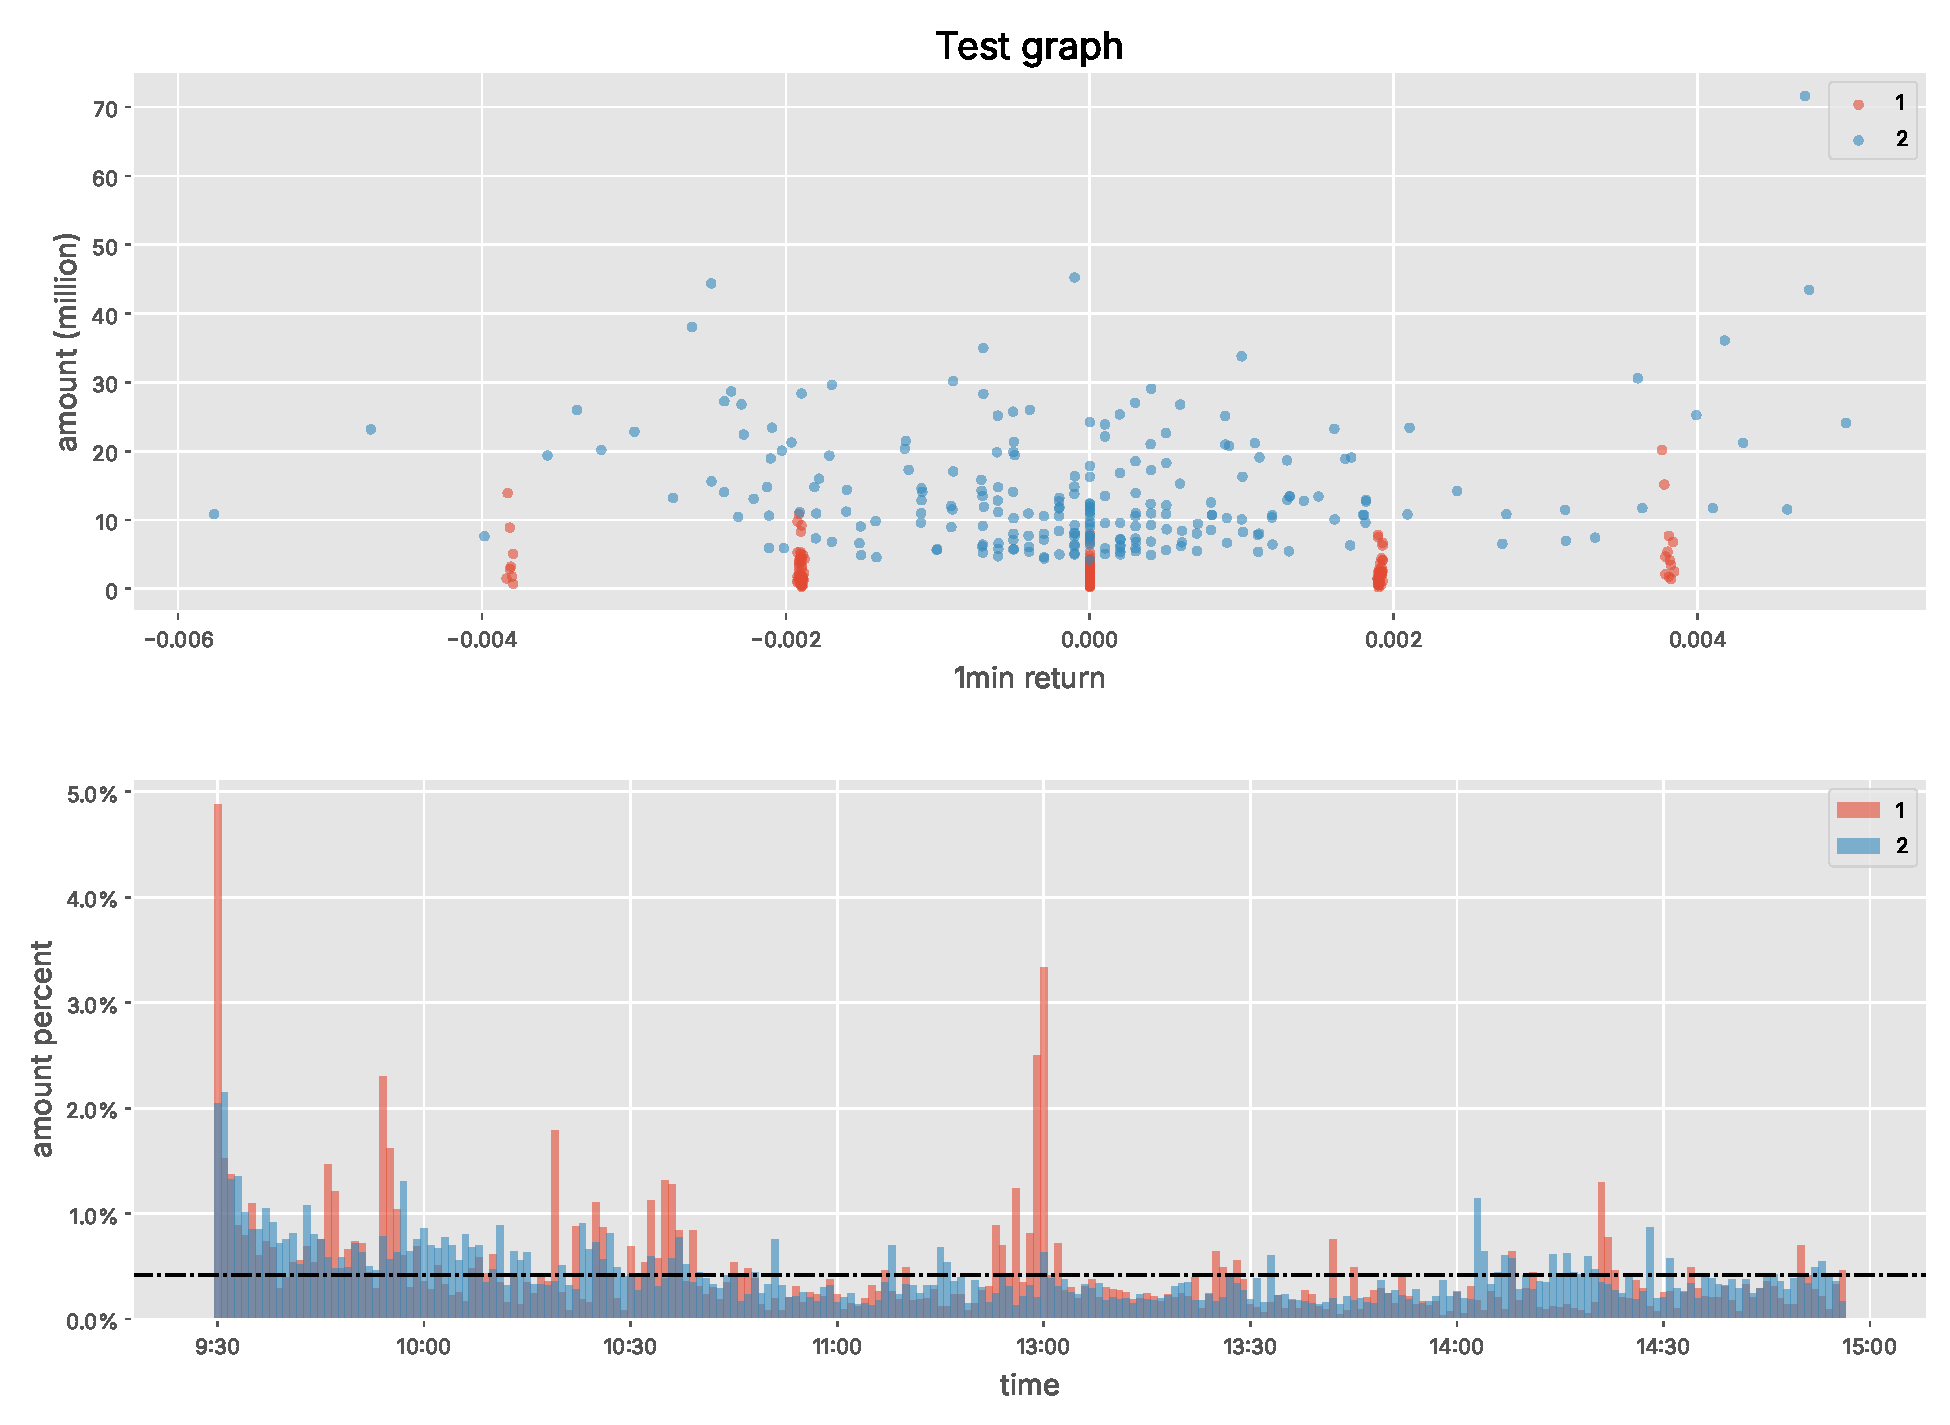
\includegraphics[width=\textwidth]{figs/q7_replica.pdf}
\caption{\Q{7} Upper panel: one-minute return against one-minute turnover (CNY million).
Lower panel: share of daily turnover traded in each minute; the dash-dotted line marks the uniform
benchmark $1/237$. Stocks~1 (red) and~2 (blue), 2021-01-04. Bins are defined as in \Q{6}.}
\label{fig:q7}
\end{figure}

\paragraph{\Q{7a} Return versus turnover.} The two stocks look very different because of the tick
grid. One tick is $0.01/5.23\approx0.19\%$ of stock~1's price, so its one-minute returns fall on a
lattice of about $0,\pm0.0019,\pm0.0038$: only 38 distinct values, and 45\% of minutes have no price
change at all. Stock~2's tick is about 1\,bp, so its returns look nearly continuous (8\% zero
minutes). For both stocks, turnover increases with the size of the price move. The correlation
between $|r|$ and turnover is 0.34 (stock~1) and 0.37 (stock~2). This is the well-documented
positive relation between volume and absolute price changes \citep{karpoff1987,jain1988}. The
cloud is roughly symmetric, i.e.\ heavy trading goes with large moves in either direction.

\paragraph{\Q{7b} Intraday distribution of turnover.} Activity is concentrated in the opening
minutes. The first bar alone accounts for 4.9\% (stock~1) and 2.0\% (stock~2) of daily turnover,
roughly 12 and 5 times the uniform benchmark. The first 30 minutes account for 28.9\% and 26.1\%,
against 12.7\% if turnover were spread evenly. Activity then decays towards the uniform level
before lunch. Stock~1 has a second spike around the break (2.5\% at 11:29 and 3.3\% at 13:00). Stock~2
picks up again after about 14:00. The last 30 minutes carry only 7.8\% and 10.8\%. The usual
end-of-day peak of the intraday ``U-shape'' \citep{wood1985,jain1988,admati1988} is missing here because the
closing call auction (14:57--15:00) is outside the sample. What remains is an L-shape with an
afternoon recovery.

\paragraph{Note on the reference image.} With the right-closed bins required by \Q{6}, our bar
heights differ slightly from those in the reference image (e.g.\ 4.88\% instead of about 4.47\% for
stock~1 at 9:30). If we use \emph{left}-closed bins $[t, t+1\,\text{min})$ instead, we reproduce
the reference values: 4.47\% at 9:30 and 3.22\% at 13:00 for stock~1, and 1.81\%/1.73\% for the top
two bars of stock~2. This indicates that the reference was built with left-closed bins.
Figure~\ref{fig:q7left} in the Appendix shows this variant. We keep the right-closed definition in
the main text because it is the one the task specifies.

%==========================================================================================
\section{Where does the last price sit in the book? (Question 8)}\label{sec:category}

\subsection*{\Q{8a} Classification and proportions}

Each snapshot with a valid \code{last} (71{,}025 of 71{,}085) is assigned a category
$c\in\{-5,\dots,5\}$ following the definition in the task:
$c=0$ if $\text{bid1p}<\text{last}<\text{ask1p}$;
$c=-i$ if $\text{bid}_{i+1}\text{p}<\text{last}\le\text{bid}_i\text{p}$ and
$c=i$ if $\text{ask}_i\text{p}\le\text{last}<\text{ask}_{i+1}\text{p}$ for $i=1,\dots,4$;
and $c=\mp5$ beyond the fifth level. The comparisons are done in integer ticks, and the script
checks that every snapshot falls into exactly one category. Table~\ref{tab:q8} gives the
proportions of each category by stock.

\begin{table}[H]
\centering\small
\caption{\Q{8a} Proportion (\%) of snapshots in each last-price category, all snapshots
(forward-filled \code{last}).}
\label{tab:q8}
\begin{adjustbox}{max width=\textwidth}
\begin{tabular}{lrrrrrrrrrrr}
\toprule
Stock & -5 & -4 & -3 & -2 & -1 & 0 & +1 & +2 & +3 & +4 & +5 \\
\midrule
Stock 1 & 0.00 & 0.00 & 0.06 & 1.53 & 52.03 & 1.04 & 44.01 & 1.32 & 0.01 & 0.00 & 0.00 \\
Stock 2 & 4.02 & 2.76 & 5.21 & 9.82 & 23.88 & 8.88 & 23.99 & 9.77 & 5.36 & 2.84 & 3.48 \\
Stock 3 & 0.49 & 0.69 & 2.15 & 7.72 & 35.19 & 1.47 & 40.16 & 9.07 & 2.21 & 0.65 & 0.20 \\
Stock 4 & 0.10 & 0.14 & 1.22 & 7.33 & 41.56 & 4.33 & 37.57 & 6.47 & 0.96 & 0.23 & 0.08 \\
Stock 5 & 12.17 & 3.95 & 5.46 & 7.47 & 17.35 & 7.22 & 20.10 & 8.19 & 5.07 & 4.00 & 9.02 \\
\bottomrule
\end{tabular}

\end{adjustbox}
\end{table}

\subsection*{\Q{8b} Line chart and findings}

\begin{figure}[H]
\centering
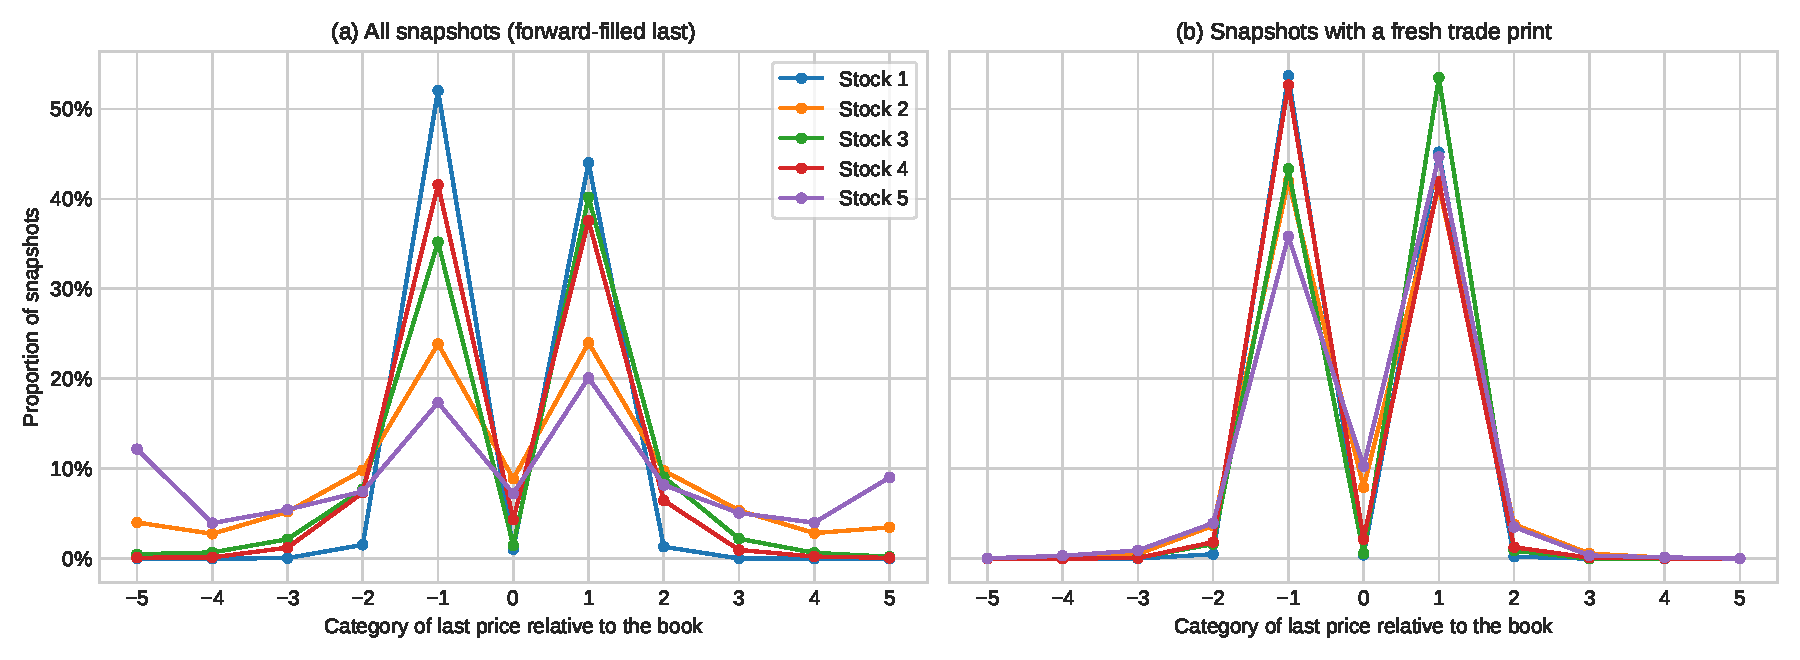
\includegraphics[width=\textwidth]{figs/q8_category.pdf}
\caption{\Q{8b} Proportion of snapshots by last-price category. Panel (a) is the requested
chart (all snapshots). Panel (b) is a robustness check that keeps only the snapshots at which a new
trade record arrives, so that \code{last} is not stale.}
\label{fig:q8}
\end{figure}

\begin{table}[H]
\centering\small
\caption{Robustness: proportion (\%) of categories using only snapshots with a fresh trade print
(14{,}205 observations).}
\label{tab:q8fresh}
\begin{adjustbox}{max width=\textwidth}
\begin{tabular}{lrrrrrrrrrrr}
\toprule
Stock & -5 & -4 & -3 & -2 & -1 & 0 & +1 & +2 & +3 & +4 & +5 \\
\midrule
Stock 1 & 0.00 & 0.00 & 0.00 & 0.49 & 53.68 & 0.42 & 45.20 & 0.21 & 0.00 & 0.00 & 0.00 \\
Stock 2 & 0.04 & 0.04 & 0.49 & 3.66 & 41.99 & 7.92 & 41.39 & 3.80 & 0.56 & 0.11 & 0.00 \\
Stock 3 & 0.00 & 0.00 & 0.11 & 1.62 & 43.33 & 0.56 & 53.47 & 0.88 & 0.00 & 0.04 & 0.00 \\
Stock 4 & 0.00 & 0.00 & 0.07 & 1.83 & 52.66 & 2.15 & 41.89 & 1.27 & 0.11 & 0.04 & 0.00 \\
Stock 5 & 0.04 & 0.32 & 0.92 & 3.94 & 35.83 & 10.28 & 44.67 & 3.52 & 0.35 & 0.14 & 0.00 \\
\bottomrule
\end{tabular}

\end{adjustbox}
\end{table}

\begin{enumerate}[leftmargin=*,itemsep=2pt]
\item \textbf{Trades happen at the touch.} Every curve peaks at $\pm1$, i.e.\ the last price
equals the best bid or the best ask. This is expected in a continuous limit-order market: a
marketable order executes against the best opposite quote, so the last price is usually a
quote price. The quote rule of \citet{lee1991} relies on exactly this property to sign trades.
Using fresh prints only (Table~\ref{tab:q8fresh}), the share at $\pm1$ is 99\% for stock~1,
95--97\% for stocks~3 and~4, and 80--83\% for stocks~2 and~5.

\item \textbf{The shape is governed by relative tick size.} The large-tick stock~1 is almost a
two-point distribution (96\% at $\pm1$). Its spread is nearly always one tick, so there is no price
strictly inside the spread and $c=0$ is practically impossible (1.0\%). For the small-tick
stocks~2 and~5, only 48\% and 37\% of snapshots are at $\pm1$, $c=0$ reaches 7--9\%, and the
tails are heavy. For stock~5, 12\% of snapshots are at $-5$ and 9\% at $+5$. Stocks~3 and~4 lie in
between (75\% and 79\% at $\pm1$).

\item \textbf{Most of the tail mass is caused by staleness.} Between two trade prints the book
keeps moving while \code{last} is held fixed for up to 15 seconds. For a small-tick stock a
15-second price move covers many ticks, so the frozen price drifts deep into the book. Restricting
to fresh prints makes the share outside $\pm1$ collapse (stock~5: from 55\% to 9\%; stock~2: from
43\% to 9\%). The tails in panel~(a) therefore measure how far the quotes move within 15 seconds,
not trades executed deep in the book.

\item \textbf{$c=0$ signals queue depletion.} A fresh print strictly inside the spread
(8--10\% for stocks~2 and~5) occurs when the last trade emptied the price level it hit, so the
next quote is at least one tick further away. This is the same one-sided depletion mechanism seen
in \Q{3b}. Such inside-spread prints are also the case that quote-based trade classification
handles least well \citep{lee1991}.

\item \textbf{Mild asymmetry.} The bid and ask sides carry similar mass. The small differences
(e.g.\ stock~1: 52\% at $-1$ versus 44\% at $+1$; stock~3: 43\% versus 53\% among fresh prints)
reflect the net direction of order flow over the three days rather than any structural bias.
\end{enumerate}

%==========================================================================================
\section{Free-hole additions (Question 9)}\label{sec:freehole}

\paragraph{Detection.} Take two consecutive snapshots of the same stock-day. On the bid side, a
price $p$ shown in the current snapshot at level $k$ is a free-hole addition if
(i)~$\text{bid5p}^{\text{prev}}<p<\text{bid1p}^{\text{prev}}$,
(ii)~$p$ is not one of the five bid prices of the previous snapshot, and
(iii)~$\text{bid}_k\text{q}>0$. The ask side is treated symmetrically, with
$\text{ask1p}^{\text{prev}}<p<\text{ask5p}^{\text{prev}}$. Condition~(ii) is exact: the five
displayed levels are the five best \emph{non-empty} prices, so a price inside the previous
displayed range that is not shown must have had zero depth. Its \emph{size in front} is the volume
queued at better prices in the current snapshot, $\sum_{j<k}\text{bid}_j\text{q}$ (zero at level 1).
As a unit test, the script runs the detector on the worked example in the task. It finds 21.17
(level 5, sizeInFront 27{,}500), 21.18 (level 4, 25{,}200) and 21.26 (ask level 2, 1{,}400), and it
correctly does \emph{not} flag the new best bid at 21.22.

\subsection*{\Q{9a} Counts by price level}

The full dataset contains \textbf{17{,}925} free-hole additions: 9{,}811 on the bid side and
8{,}114 on the ask side. Table~\ref{tab:q9a} gives the breakdown by level.

\begin{table}[H]
\centering\small
\caption{\Q{9a} Number of free-hole additions by price level (level in the \emph{current}
snapshot).}
\label{tab:q9a}
\begin{tabular}{lrrrr}
\toprule
Price level & Bid side & Ask side & Total & Share (\%) \\
\midrule
Level 1 & 1{,}604 & 1{,}261 & 2{,}865 & 16.0 \\
Level 2 & 2{,}485 & 2{,}193 & 4{,}678 & 26.1 \\
Level 3 & 2{,}362 & 1{,}931 & 4{,}293 & 23.9 \\
Level 4 & 1{,}902 & 1{,}515 & 3{,}417 & 19.1 \\
Level 5 & 1{,}458 & 1{,}214 & 2{,}672 & 14.9 \\
Total & 9{,}811 & 8{,}114 & 17{,}925 & 100.0 \\
\bottomrule
\end{tabular}

\end{table}

Level~2 is the most frequent (26\%), followed by levels~3 (24\%) and~4 (19\%). Additions at
level~1 (16\%) happen when the previous best level has disappeared and the new best quote is a
price that was previously empty, i.e.\ the inside of the book refills at a new price. The
distribution is close to symmetric between bid and ask at every level.

\begin{table}[H]
\centering\small
\caption{Free-hole additions by stock. ``Mean holes in book'' is the average number of empty tick
prices strictly inside the displayed five levels (both sides combined).}
\label{tab:q9stock}
\begin{adjustbox}{max width=\textwidth}
\begin{tabular}{lrrrrrrrr}
\toprule
Stock & L1 & L2 & L3 & L4 & L5 & Total & Per 1,000 snaps & Mean holes in book \\
\midrule
Stock 1 & 0 & 2 & 0 & 0 & 0 & 2 & 0.14 & 0.00 \\
Stock 2 & 1{,}176 & 1{,}892 & 1{,}573 & 1{,}160 & 791 & 6{,}592 & 463.77 & 5.73 \\
Stock 3 & 102 & 197 & 133 & 47 & 28 & 507 & 35.67 & 0.11 \\
Stock 4 & 108 & 160 & 65 & 29 & 16 & 378 & 26.59 & 0.31 \\
Stock 5 & 1{,}479 & 2{,}427 & 2{,}522 & 2{,}181 & 1{,}837 & 10{,}446 & 734.91 & 15.32 \\
\bottomrule
\end{tabular}

\end{adjustbox}
\end{table}

Table~\ref{tab:q9stock} shows that the counts are extremely uneven across stocks. Stocks~5 and~2
account for 10{,}446 and 6{,}592 additions (0.73 and 0.46 per snapshot), while stock~1 has only~2.
The reason is mechanical: a free hole can only be filled if one exists. The displayed books of the
small-tick stocks contain on average 15.3 and 5.7 empty interior ticks, whereas the book of stock~1
is essentially dense (0.0002 empty ticks on average). On a large-tick stock every price close to the
touch already holds a queue, so a new order joins an existing queue instead of opening a new level.

\subsection*{\Q{9b} Size in front}

\begin{table}[H]
\centering\small
\caption{\Q{9b} Percentiles of \code{sizeInFront} (shares). The stock~1 row is based on two
events and is reported only for completeness.}
\label{tab:q9b}
\begin{tabular}{lrrrrrr}
\toprule
Sample & 10\% & 30\% & 50\% & 70\% & 90\% & N \\
\midrule
All additions & 0 & 600 & 2{,}100 & 5{,}000 & 14{,}900 & 17{,}925 \\
Bid side & 0 & 600 & 2{,}000 & 4{,}700 & 14{,}400 & 9{,}811 \\
Ask side & 0 & 700 & 2{,}300 & 5{,}400 & 15{,}300 & 8{,}114 \\
Excluding level 1 & 400 & 1{,}400 & 3{,}000 & 6{,}100 & 17{,}000 & 15{,}060 \\
Stock 1 & 36{,}427 & 50{,}482 & 64{,}536 & 78{,}591 & 92{,}646 & 2 \\
Stock 2 & 0 & 500 & 1{,}800 & 4{,}400 & 13{,}651 & 6{,}592 \\
Stock 3 & 0 & 2{,}580 & 9{,}400 & 22{,}580 & 87{,}520 & 507 \\
Stock 4 & 0 & 300 & 5{,}150 & 16{,}670 & 61{,}930 & 378 \\
Stock 5 & 0 & 700 & 2{,}200 & 4{,}900 & 13{,}200 & 10{,}446 \\
\bottomrule
\end{tabular}

\end{table}

For the full sample, the 10th, 30th, 50th, 70th and 90th percentiles of \code{sizeInFront} are
\textbf{0, 600, 2{,}100, 5{,}000 and 14{,}900 shares} (Table~\ref{tab:q9b}). The lower tail is zero
because of the level-1 additions; without them the percentiles are 400, 1{,}400, 3{,}000, 6{,}100
and 17{,}000 shares. The distribution is strongly right-skewed and very similar on the bid and ask
sides. Since stocks~2 and~5 dominate the sample, the pooled figures largely describe those two
names. For stocks~3 and~4 the median queue ahead is larger (9{,}400 and 5{,}150 shares), in line
with their lower prices and thicker queues.

The economic interpretation is that free-hole additions are \emph{price-improving placements
behind a thin queue}. A trader who posts at an empty interior price gets ahead of all the volume
resting at worse prices, at the cost of a small amount of price improvement (typically one level
behind the best quote). \citet{biais1995} document the same behaviour on the Paris Bourse: when the spread or the depth
at the quotes is large, investors quickly place orders within the quotes to gain price and time
priority. In the high-priced stocks, where empty ticks are common and a tick is
cheap in relative terms, this is an inexpensive way to gain priority, and the new orders are
typically small (median 300 shares for stocks~2 and~5). This links queue position to the
relative tick size, as discussed by \citet{dayri2015} and \citet{bouchaud2018}.

%==========================================================================================
\section{Conclusion}\label{sec:conclusion}

A single variable, the relative tick size, organises almost all of the results. In the large-tick
stocks the spread is pinned at one tick, widenings are rare and one-sided, trades print exactly at
the touch, and the book has no gaps to fill. In the small-tick stocks the spread is wide and often
widening, the forward-filled last price wanders through the book between prints, and new orders
are frequently placed in empty price levels with little volume ahead of them. Turnover is
concentrated at the open and co-moves with absolute returns, in line with the classical intraday
evidence.

\paragraph{Limitations.} The sample covers only three days and five stocks, so the
cross-sectional patterns should be read as descriptive. With 3-second snapshots, any events that
cancel out between two snapshots are invisible (for example, a hole that is filled and emptied
again), so free-hole counts are lower bounds. Trade records are aggregated over 15 seconds, so
\code{last} is stale most of the time, which matters for \Q{5b} and \Q{8}. Finally, the closing
auction is not in the data, which affects the shape of the intraday profile in \Q{7b}.

%==========================================================================================
\newcommand{\doi}[1]{\href{https://doi.org/#1}{doi:#1}}
\begin{thebibliography}{99}\setlength{\itemsep}{1pt}\small

\bibitem[Admati and Pfleiderer(1988)]{admati1988}
Admati, A.~R. and Pfleiderer, P. (1988). A theory of intraday patterns: Volume and price
variability. \emph{Review of Financial Studies}, 1(1):3--40. \doi{10.1093/rfs/1.1.3}

\bibitem[Biais et~al.(1995)]{biais1995}
Biais, B., Hillion, P. and Spatt, C. (1995). An empirical analysis of the limit order book and the
order flow in the Paris Bourse. \emph{Journal of Finance}, 50(5):1655--1689.

\bibitem[Bouchaud et~al.(2018)]{bouchaud2018}
Bouchaud, J.-P., Bonart, J., Donier, J. and Gould, M. (2018). \emph{Trades, Quotes and Prices:
Financial Markets Under the Microscope}. Cambridge University Press. \doi{10.1017/9781316659335}

\bibitem[Dayri and Rosenbaum(2015)]{dayri2015}
Dayri, K. and Rosenbaum, M. (2015). Large tick assets: Implicit spread and optimal tick size.
\emph{Market Microstructure and Liquidity}, 1(1):1550003. arXiv:1207.6325.

\bibitem[Eisler et~al.(2012)]{eisler2012}
Eisler, Z., Bouchaud, J.-P. and Kockelkoren, J. (2012). The price impact of order book events:
Market orders, limit orders and cancellations. \emph{Quantitative Finance}, 12(9):1395--1419.
\doi{10.1080/14697688.2010.528444}

\bibitem[Harris(1994)]{harris1994}
Harris, L. (1994). Minimum price variations, discrete bid--ask spreads, and quotation sizes.
\emph{Review of Financial Studies}, 7(1):149--178. \doi{10.1093/rfs/7.1.149}

\bibitem[Jain and Joh(1988)]{jain1988}
Jain, P.~C. and Joh, G.-H. (1988). The dependence between hourly prices and trading volume.
\emph{Journal of Financial and Quantitative Analysis}, 23(3):269--283. \doi{10.2307/2331067}

\bibitem[Karpoff(1987)]{karpoff1987}
Karpoff, J.~M. (1987). The relation between price changes and trading volume: A survey.
\emph{Journal of Financial and Quantitative Analysis}, 22(1):109--126.

\bibitem[Lee and Ready(1991)]{lee1991}
Lee, C.~M.~C. and Ready, M.~J. (1991). Inferring trade direction from intraday data.
\emph{Journal of Finance}, 46(2):733--746. \doi{10.2307/2328845}

\bibitem[Wood et~al.(1985)]{wood1985}
Wood, R.~A., McInish, T.~H. and Ord, J.~K. (1985). An investigation of transactions data for NYSE
stocks. \emph{Journal of Finance}, 40(3):723--739. \doi{10.2307/2327796}

\end{thebibliography}

%==========================================================================================
\clearpage
\appendix
\section{Supplementary material}\label{app}

\subsection*{A.1\quad Reference-consistent version of Figure~\ref{fig:q7}}

\begin{figure}[H]
\centering
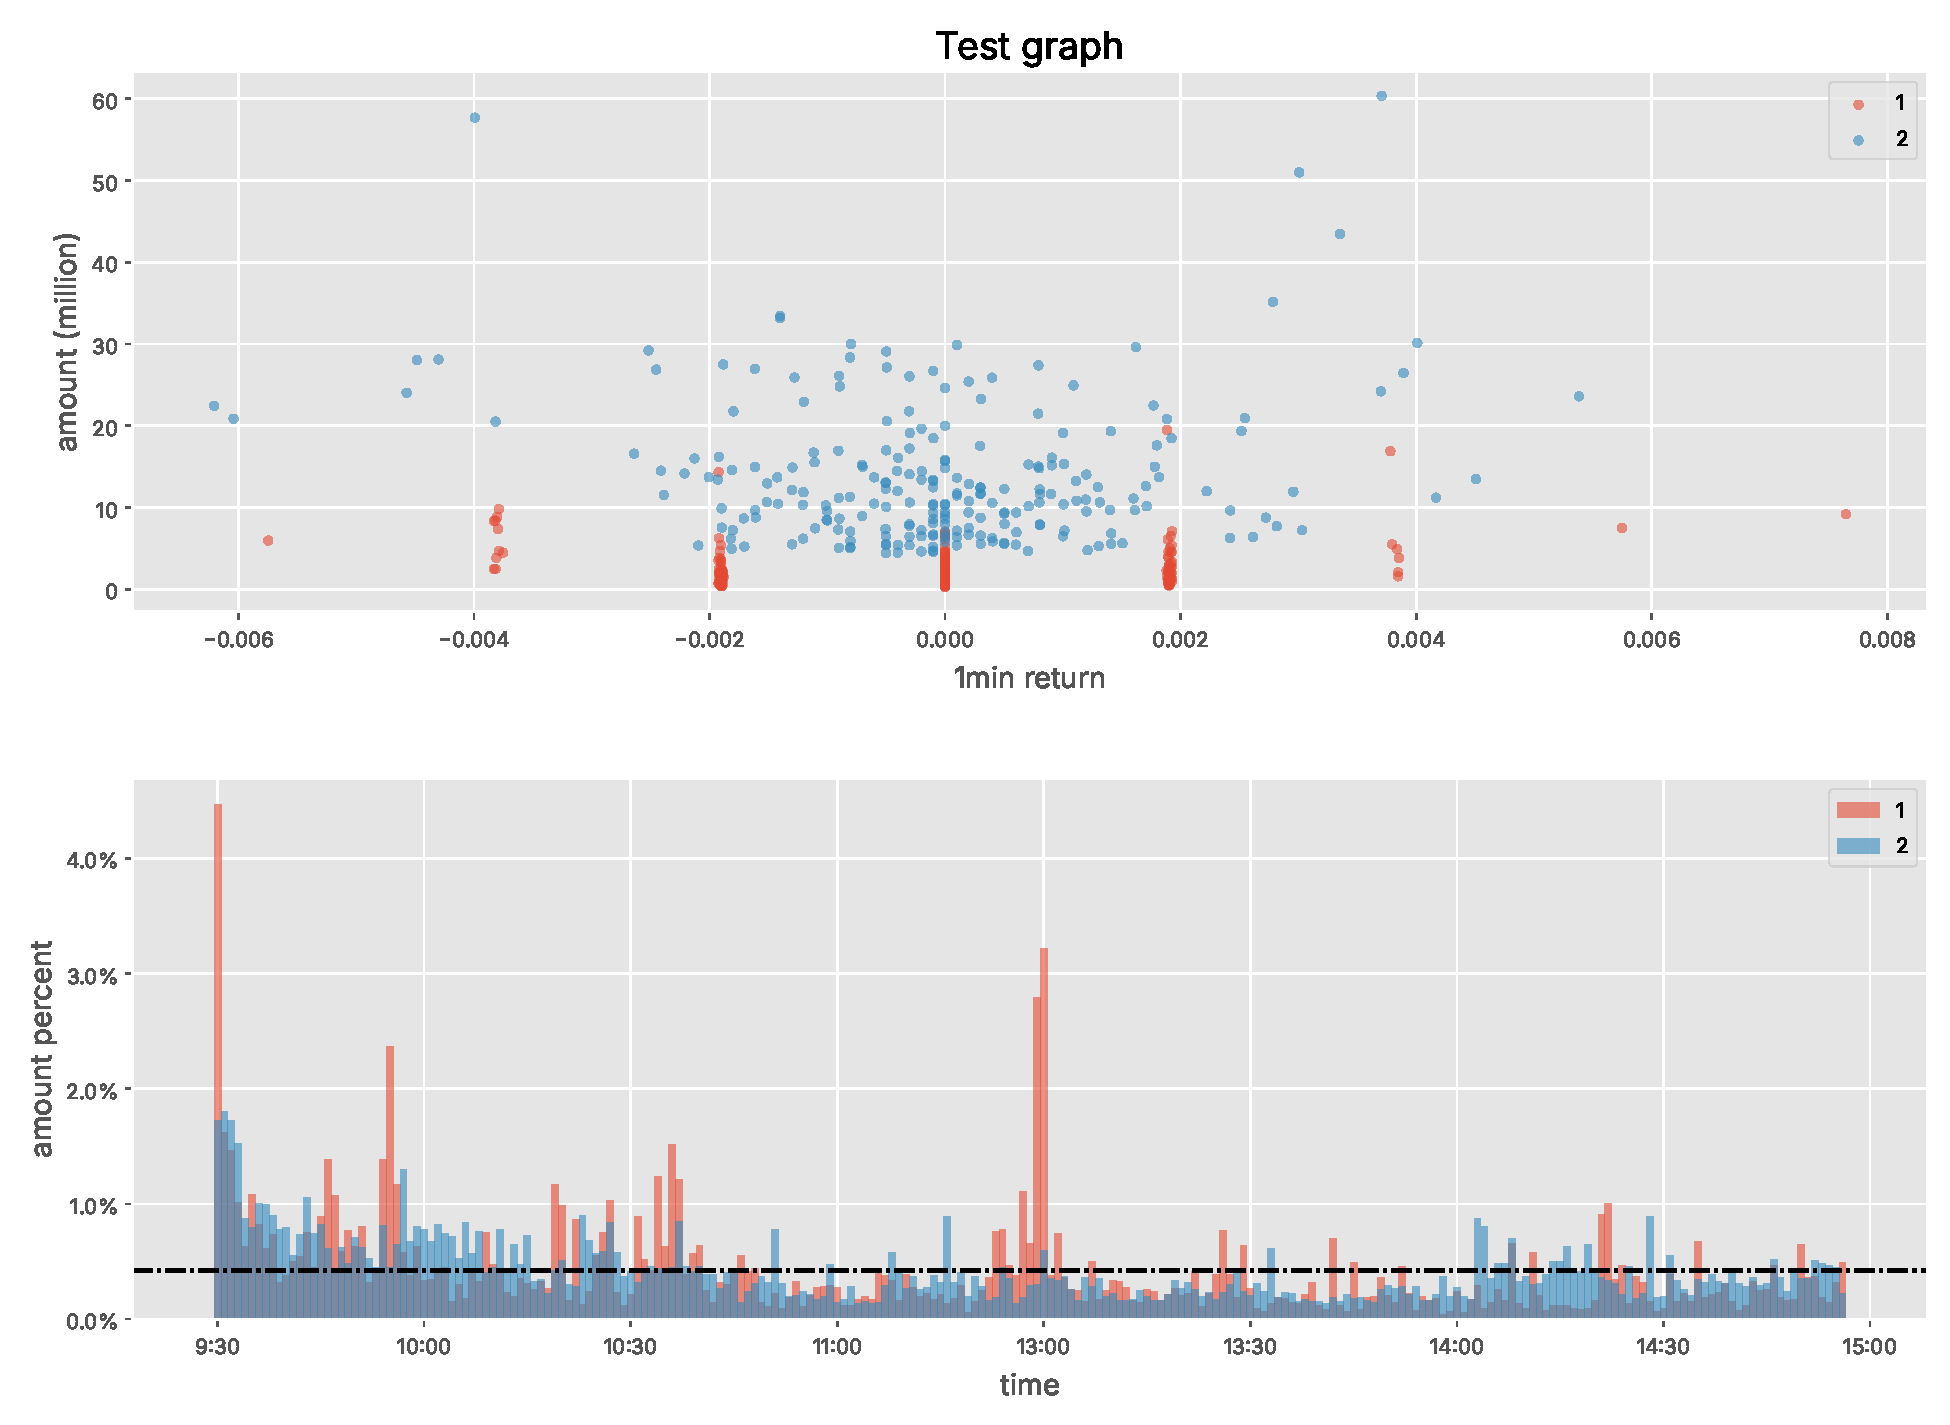
\includegraphics[width=\textwidth]{figs/q7_leftclosed.pdf}
\caption{Same chart as Figure~\ref{fig:q7}, but with left-closed one-minute bins $[t,t+1\,\text{min})$
labelled by $t$ (the lone 11:30:00 snapshot is folded into the 11:29 bar so that there are 237 bars).
With this convention the bar heights match the reference image provided with the task.}
\label{fig:q7left}
\end{figure}

\subsection*{A.2\quad Reproducibility}

The entire analysis is in one script:
\begin{lstlisting}[language=bash]
python analysis.py --data <folder containing snapshot/ and trade/> --out <output folder>
\end{lstlisting}
It runs in under a minute on a laptop (pandas~3.0, NumPy, Matplotlib). It writes every table in
this report (\code{tables/*.tex}), every figure (\code{figs/}), the intermediate snapshot-level and
one-minute data frames, the list of free-hole additions, and a \code{results.json} file with the
numbers quoted in the text. The integrity checks of Section~\ref{sec:data} and the cross-checks
described in Sections~\ref{sec:assembly}--\ref{sec:freehole} are written as assertions, so the
script stops if any of them fails.

\end{document}
